
%
%  $Description: Two variants of a distributed fault-tolerant Tuple Space system$ 
%
%  $Author: Mafalda Ferreira, Leonardo Epifânio and Pedro Lopes $
%  $Date: 2018/12/09 15:20:59 $
%  $Revision: 1.0 $
%

\documentclass[times, 10pt,twocolumn]{article} 
\usepackage{latex8}
\usepackage{times}
\usepackage{graphicx}
\usepackage{framed}
\usepackage{caption}
\usepackage{lastpage}
\usepackage{fancyhdr} 

\renewcommand{\headrulewidth}{0pt}
\fancyhf{}
\cfoot{\number\value{page} of \pageref{LastPage} pages}
\pagestyle{fancy} 

\graphicspath{ {./images/} }

%------------------------------------------------------------------------- 
% take the % away on next line to produce the final camera-ready version 
\pagestyle{empty}

%------------------------------------------------------------------------- 
\begin{document}

\title{ Two variants of a distributed fault-tolerant Tuple Space system}

\author{Mafalda Ferreira, Leonardo Epif\^{a}nio and Pedro Lopes\\
Instituto Superior T\'{e}cnico\\ 
Av. Rovisco Pais 1, 1049-001 Lisbon\\
DIDA 18/19 (MEIC-A / MEIC-T / METI)\\
Group 4
}

\maketitle
\thispagestyle{empty}

\begin{abstract}
   We describe the developed solution for the implementation of two variants
   of a distributed fault-tolerant Tuple Space system: State Machine Replication~\cite{Bakken:1995:SFP:203121.203132} and Xu-Liskov~\cite{Xu1989ADF}. 
   This paper outlines the key design philosophies and explanation of the 
   algorithms used in each variant. We discuss the relative advantages of each solution,
   and present experimental results.
\end{abstract}

%------------------------------------------------------------------------- 
\Section{Introduction} \label{introduction}

A Tuple Space (referred to as TS from this point on) is an approach to shared memory systems, where the processes involved 
communicate indirectly by placing tuples in a TS. A tuple 
can be accessed and removed by pattern matching. Most implementations use a 
centralized solution where the TS is managed by a single server. This is a simple 
solution but has several restrictions. It doesn't scale, being more prone to availability issues, and it is also not fault tolerant, since there's a single point of failure. 

Distributed systems are interesting for four main reasons: scalability, high performance, 
availability and reliability. However, implementing a distributed system rises many issues. The computing 
nodes can crash, messages can be lost, duplicated or delivered out of order and the network 
can fail. If we don't take these issues into consideration, the system as a whole can fail.

This paper presents two design variants of a fault-tolerant, distributed system for a 
TS where high availability and fault tolerance are achieved with replication in several nodes. 
The main challenge with replication is maintaining data consistency among replicas. To surpass
this issue, we consider the two following variants:

\begin{itemize}
  \item The first variant is called State Machine Replication~\cite{Bakken:1995:SFP:203121.203132} 
  (referred to as SMR from this point on) and it's based on the approach in which the TS 
  behaves like a state machine, maintaining state and changing it deterministically, 
  in response to events received. In order to ensure consistency between replicas, it is required
  that the replicas must start in the same state and must execute events in the same order. 
  To satisfy the second requirement, we will adopt a total order algorithm.
  
  \item The second variant is based in the Xu-Liskov implementation~\cite{Xu1989ADF} (referred to as 
  XL from now on) which is designed to minimize delay of responses, given the semantics of the three TS
  operations: \textit{add}, \textit{read} and \textit{take}. In this approach, the consistency in the \textit{take} operation is assured
  by the agreement of the replicas on the tuple to be selected, and removing this tuple from all replicas.
\end{itemize}

We begin in section \ref{design} by briefly describing the implementation tools and the main 
design and architecture of the solution. Section \ref{overview} gives an overview of the common
parts in the two variants, including leader election, how a replica joins the view, and the perfect and 
imperfect failure detector. Both variants will be described in more detail in sections 
\ref{smr}, \ref{xl} and \ref{client_failure}. In Section \ref{evaluation} we'll discuss the relative advantages of each variant and present experimental results. The conclusion is then presented in section \ref{conclusion}.

%------------------------------------------------------------------------- 
\Section{Design and Architecture} \label{design}

The solution was implemented in C\# and .Net Remoting using Microsoft Visual Studio and the 
OOP paradigm.

%------------------------------------------------------------------------- 
\SubSection{Architecture}
\begin{figure}[h]
\centering
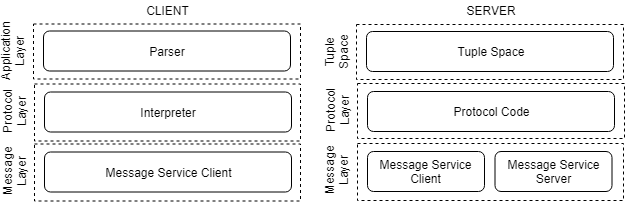
\includegraphics[width=1\linewidth]{dad_architecture.png}
\caption{Layered architecture of the client and server.}
\label{fig:architecture}
\end{figure}

For the client and server we chose a layered architecture and a modular design for simplicity
in development as we can see in the figure \ref{fig:architecture}. 

The module \textit{Message Service Client} has two methods: \textit{Request} and \textit{Multicast}. Both call 
the remote method \textit{Request} of the module \textit{Message Service Server}. The Message Layer receives the messages and passes them to the Protocol Layer where the system protocol runs. 
In the case of the server, the Protocol Layer calls the Tuple Space module to conclude
the operations over the TS in the replica.

Each layer has a clean API that can be called by the under layer. The requests and
responses correspond to serialized objects that are processed in the Protocol Layer
using the Visitor design pattern.

%------------------------------------------------------------------------- 
\Section{Overview} \label{overview}
Both variants have the following different status: \textsc{Initialization}, \textsc{ViewChange} and
\textsc{Normal}. The SMR has one extra status, which is \textsc{Recovery}. The server only 
processes requests when in the \textsc{Normal} status. The behaviours in each state are detailed in the succeeding sections.

Despite the differences between the two, they share some of the problems that
are inherited from the development of distributed systems. All replicas must agree on the 
current view, they must detect failures and, consequentially, must all act the same
way. Messages can be duplicated, therefore, they must be filtered. Delays can also happen and messages can arrive out of order.

%------------------------------------------------------------------------- 
\SubSection{Filter Duplicate Messages} \label{filter_duplicates}
Each replica has a Client Table which saves, for each client, the client-id of the last request, the request number
and the respective response. The algorithm to filter duplicates works as follows:
\begin{enumerate}
  \item The client sends the message 
  $\left \langle   \textsc{Request} \: \: op, \: c, \: s \right \rangle$ where
 \textit{op} is the \textit{operation} with its arguments, \textit{c} is the \textit{client-id} and \textit{s} is the \textit{request-number} assigned to the request (which is an incremented counter
 starting at 0).
  \item When the server receives the message, it compares the \textit{request-number} with
  the information in the Client Table (on the row that corresponds to the client that sent it). If the \textit{request-number} is smaller than the
  \textit{request-number} in the Client Table, it drops it. If it's equal, it re-sends 
  the response that is stored in the Client Table, otherwise it accepts and processes the request.
\end{enumerate}

%------------------------------------------------------------------------- 
\SubSection{View Changes} \label{view_change}
Although the information passed in the messages about the replica's state is different for each variant, the semantic of the messages remains. A configuration can be seen as group of $2f + 1$ replicas. The algorithm is as follows:

\begin{enumerate}
  \item When a replica $i$ notices the need for a view change, it sets its status
  to \textit{ViewChange} and sends the message 
  $\left \langle   \textsc{StartViewChange} \: \: i, \: v, \: c \right \rangle$ 
  to all  the other replicas, where $v$ is the new \textit{view-number} and $c$ is the new 
  \textit{configuration}.
  
  \item When a replica $i$ receives $f$ \textsc{StartViewChange} messages for its \textit{view-number}
  and \textit{configuration}, it sends $\left \langle   \textsc{DoViewChange} \: \: i, \: v, \: v', \: c, \: s, \: k \right \rangle$ to the node that will be the leader in the new view, where $v'$ is the previous view-number, $s$ is the state of the replica and $k$ is the commit number.
  
 \textbf{In SMR:} $s=\left ( l, \: n \right )$, where $l$ is the logger and $n$ is the op-number.
 
  \textbf{In XL:} $s=\left ( t, \: d \right )$, where $t$ is the TS and $d$ is the Client Table.
  
  \item When the new leader receives $f + 1$ \textsc{DoViewChange} messages, it selects the best state
  and updates its state, then informs all the other replicas by sending the message 
  $\left \langle   \textsc{StartChange} \: \: i, \: v, \: c, \: s, \: k \right \rangle$
  and sets its status back to \textit{Normal}. The best state is the one with the biggest view-number. 
  In case of a draw, it selects the biggest op-number and the biggest commit-number in 
  SMR and XL respectively.
  The replicas that receive the \textsc{StartChange} message, update their state.
 
\end{enumerate}

In the case of SMR, there are two extra steps:
\begin{enumerate}
  \setcounter{enumi}{3}
  \item The new leader starts accepting client requests. It also executes (in order) 
  any committed operations that it hadn’t executed previously and updates the Client Table.
  
  \item When the other replicas receive \textsc{StartChange}, they update their state and
  set the status back to \textit{Normal}. If there are non-committed operations in the log, they
  send a \textsc{PrepareOk} to the leader. Then execute, in order, all operations known
  to be commited.
\end{enumerate}

%------------------------------------------------------------------------- 
\SubSection{Leader Election} \label{leader_election}
The leader of a configuration is the first server-id in lexicographical order. Thus,
when a configuration is agreed upon in the view-change, the leader is implicitly elected.
The leader in SMR also becomes the primary.

%------------------------------------------------------------------------- 
\SubSection{Initialization Operation} \label{init}
When a replica starts up or thinks that it's out of the current view, the status is changed to \textit{Initialization}. The protocol runs as following:
\begin{enumerate}
  \item A replica $i$ sends, to a all possible servers, the message $\left \langle \textsc{ServerHandShake} \: \: i \right \rangle$. If it doesn't receive a response in a determinate timeout, 
  it thinks that it's the first server and sets its status to \textit{Normal}.
  
  \item If one or more replicas are alive, they will respond with the current view
  configuration, and replica $i$ sends, to all servers in the 
  configuration, the message $\left \langle \textsc{JoinView} \: \: i, \: u \right \rangle$, 
  where $u$ represents the URL of the replica $i$. Then it waits for a \textsc{StartChange} message
  and updates its status as explained in section \ref{view_change}.
  If the message doesn't arrive in a determinate time span, it repeats step 1.
  
\end{enumerate}

%------------------------------------------------------------------------- 
\SubSection{Failure Detector} \label{failure_detector}
Each replica $i$ is monitored by all the other replicas in the view. Replica $i$ periodically 
sends a lease renewal request $\left \langle \textsc{HeartBeat} \: \: i \right \rangle$.
When a monitor acknowledges with $\left \langle \textsc{HeartBeatResponse} \: \: v \right \rangle$, 
where $v$ is the view number%
\footnote
   {%
     The view-number is a health check to see if replica $i$ is in the current view.
   }, 
   replica $i$ is said to obtain a lease.


%------------------------------------------------------------------------- 
\subsubsection{Perfect Failure Detector} \label{pfd}
When a replica $i$ fails to renew a lease in a replica $j$, the perfect failure detector 
says promptly that $i$ is faulty and $j$ sets its status to \textit{ViewChange} and sends the message
\textsc{StartViewChange} to everyone. The other replicas, as they receive the 
\textsc{StartViewChange} message, change their status to \textit{ViewChange} and also send the message
\textsc{StartViewChange} to everyone. From here on, the protocol runs as explained in 
section \ref{view_change}. Also, the next leader may not be aware of the detection of 
\textsc{StartViewChange} messages, but when it receives \textsc{DoViewChange}, it changes the status to
\textit{ViewChange} and the protocol proceeds.

%------------------------------------------------------------------------- 
\subsubsection{Imperfect Failure Detector} \label{ifd}
When a replica $i$ fails to renew a lease in a replica $j$, the imperfect failure detector
is conservative. It changes its status to \textit{ViewChange} and proposes a view change by sending
\textsc{StartViewChange} messages to the other replicas. However, it waits a determinate timeout for $f$ \textsc{StartViewChange} messages, confirming its view change. If it doesn't receive $f$ \textsc{StartViewChange} messages,
the change is cancelled and the replica changes the status back to \textit{Normal}. There needs to be quorum, to decide that
$i$ is faulty.

%------------------------------------------------------------------------- 
\Section{State Machine Replication} \label{smr}
The core of SMR is the implementation of a total order protocol. For this, we decided
to implement Viewstamped Replication~\cite{Oki:1988:VRN:62546.62549} since it is simple, 
correct, easy to understand and easy to implement in comparison with Paxos~\cite{Lamport:1998:PP:279227.279229} 
or Raft~\cite{Ongaro:2014:SUC:2643634.2643666}.

%------------------------------------------------------------------------- 
\SubSection{Normal Operation} \label{smr_normal}
\fbox{\begin{minipage}{22em}
\begin{itemize}
  \item \textbf{\textit{op-number}:} assigned to the most recently received
  request, initially 0.
  \item\textbf{\textit{log}:}  This is an array containing \textit{op-number} entries. 
  The entries contain the requests that have been received so far 
  in their assigned order.
  \item \textbf{\textit{commit-number}:} is the op-number of the most
  recently committed operation.

\end{itemize}
\end{minipage}
}
\begin{figure}[h]
   \caption{State of the SMR replica.}
   \label{fig:state_smr}
\end{figure}

This section describes the process of requests that are accepted when the primary
isn't faulty. The client only communicates with the primary when performing a request.
It runs as follows:

\begin{enumerate}
  \item When the primary accepts a request, it increments its \textit{op-number}, adds the request
  to the end of the $log$ and updates the information in the client table. Then it sends
  a $\left \langle \textsc{Prepare} \: \: v, \: m, \: n, \: k \right \rangle$ to the other 
  replicas, where $m$ is the message received from the client.
  
  \item The backup replicas process the \textsc{Prepare} messages in order. They won’t accept a prepare message
  with \textit{op-number} $n$ until they have entries for all earlier requests in their $log$ (it may
  require \textit{Recovery}), putting the message on hold until the condition is met. Then 
  they increment their \textit{op-number}, add the request to the end of the $log$, update
  the client's information in the client table, and send a 
  $\left \langle \textsc{PrepareOk} \: \: v, \: n \: i\right \rangle$
  message to the primary, to indicate that this operation and all earlier ones have been
  prepared locally.
  
  \item The primary waits for $f$ \textsc{PrepareOk} messages from different backups. 
  After it receives these messages, it considers the operation (and all earlier ones) to be \textit{committed}. 
  Then, after it has executed all earlier operations (those assigned smaller \textit{op-numbers}), 
  the primary executes the operation by making an upper call to the TS, and increments its \textit{commit-number}.
  Then, it sends a $\left \langle \textsc{Reply} \: \: v, \: s, \: x\right \rangle$ message
  to the client, where $v$ is the \textit{view number}, $s$ the \textit{request-number} and $x$ the result
  of the the call to the TS. The primary saves this reply in the client table.

\begin{figure}[h]
\centering
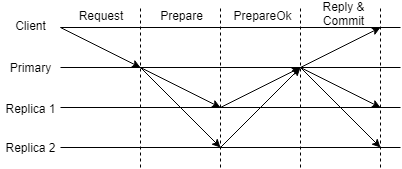
\includegraphics[width=1\linewidth]{images/dad_smr_normal.png}
\caption{Normal case processing for a configuration f=1.}
\label{fig:smr_normal_case}
\end{figure}

  \item The primary informs the other replicas about the commit, by sending a
  $\left \langle \textsc{Commit} \: \: i, \: v, \: k\right \rangle$.
  
  \item When a backup learns about the commit  it waits until it has the request in its 
  $log$ (which may require Recovery) and until it has executed all earlier operations.
  Then it executes the operation by doing an upper call to the TS, increments its \textit{commit-number}
  and updates the client table.
\end{enumerate}

Figure \ref{fig:smr_normal_case} shows the phases of the normal processing protocol.


%------------------------------------------------------------------------- 
\SubSection{Recovery Operation} \label{smr_recovery}
Recovery is used when a replica lags behind (but hasn't crashed), and needs to be brought up-to-date. After a certain time without executing anything, the 
replica changes its status to \textit{Recovery} and starts the following protocol:

\begin{enumerate}
  \item The replica $i$ sends a $\left \langle \textsc{Recovery} \: \: i, \: v, \: n', \: k\right \rangle$
  to all replicas in its configuration, where $n'$ is its \textit{op-number}.
  
  \item A replica only responds to a \textsc{Recovery} message if, and only if, its status is \textit{Normal}
  and if it's in the same view. In this case it sends a 
  $\left \langle \textsc{RecoveryResponse} \: \: v, \: n, \: k, \: l'\right \rangle$, where 
  $l'$ corresponds to its $log$ after $n'$.
  
  \item When replica $i$ receives the \textsc{RecoveryResponse} message, it appends it to
  its $log$ and updates its state using the other information in the message.
\end{enumerate}
%------------------------------------------------------------------------- 
\Section{Xu-Liskov} \label{xl}
The XL variant is simpler than SMR as it doesn't require total order. However, to maintain
consistency and simplify the implementation, we decided that the requests of the client 
should be executed in order and, thus, it respects casual order. This means that the add 
operation also blocks, and that it will not return until it gets all the acknowledge messages from the servers 
in the current configuration.

%------------------------------------------------------------------------- 
\SubSection{Normal Operation} \label{xl_normal}
\fbox{\begin{minipage}{22em}
\begin{itemize}
  \item \textbf{\textit{commit-number}:} The number of executed operations.

\end{itemize}
\end{minipage}
}
\begin{figure}[h]
   \caption{State of the XL replica.}
   \label{fig:state_xl}
\end{figure}

Besides the TS and the client table, the XL also has a \textit{commit-number} attribute as shown 
in figure \ref{fig:state_xl}.

The XL variant provides 2 more requests in addition to the three (\textit{add}, \textit{read} and \textit{take}):
\begin{itemize}
  \item \textit{\textbf{getAndLock}}: This request has an argument,
  which is the tuple pattern that the client wants to take. The response will be the set of tuples 
  that match that pattern. The server locks those tuples in the process, atomically. If the lock process
  fails, it returns a refusal response.
  
  \item \textit{\textbf{unlock}}: The request \textit{unlock} unlocks any tuple set that the client
  has locked in the moment. Also atomically.
  
\end{itemize}

In the \textit{Normal} status, when a replica accepts a request from the client (if the client sends a request 
with a smaller view number, it is dropped), it executes the operation by doing an upper call to 
the TS, advances its commit-number, updates its client table, and sends to the client the message
$\left \langle \textsc{Reply} \: \: v, \: s, \: x\right \rangle$.

%------------------------------------------------------------------------- 
\Section{Hiding failure from the client} \label{client_failure}
The biggest advantage in a fault-tolerant system, is masking the failure to the client. 
Here, it is accomplished by also saving the current view status in the client.
When the client doesn't receive  a timely response to a request, it performs a 
\textsc{ClientHandShake} to retrieve the new view and hence, in the case of SMR, retrieving the new leader. The \textsc{ClientHandShake} works as follows:
\begin{enumerate}
  \item When the client initializes or doesn't receive a timely response to a request, it sends
  $\left \langle \textsc{ClientHandShake} \: \: c \right \rangle$ to a set of possible servers,
  where $c$ is the client-id.
  
  \item The client waits (with a timeout) until receives a response 
  $\left \langle \textsc{ClientHandShakeResponse} \: \: p, \: v, \: r, \: l \right \rangle$,
  where $p$ is the protocol used by the server, $v$ is the view-number, $r$ is the configuration
  and $l$ is leader (in case of SMR). If it doesn't receive the response within the timeout period,
  step 1 is repeated.
\end{enumerate}

%------------------------------------------------------------------------- 
\Section{Evaluation} \label{evaluation}
We evaluate the performance for the different variants of the TS. We identify the relative
advantages of each implementation and show the practical results of the evaluation.

%------------------------------------------------------------------------- 
\SubSection{Detection: Perfect vs Imperfect}
In Perfect Failure Detector (PFD), when a replica suspects that a node is down, the other replicas 
trust this judgement and act accordingly. In Imperfect Failure Detector (IFD), there needs to be a quorum
of replicas suspecting that a node is faulty, in order to agree with a view change.

Although IFD is better at not excluding replicas that are not faulty (but that some of the other replicas think they are),
it brings a lot more overhead into the system and the network. In our implementation of IFD, 
explained in section \ref{ifd}, a replica can switch to status \textit{ViewChange} several times, halting 
the process of requests each time, before a view-change is accepted by a quorum, leading to a 
decrease in performance in comparison with PFD. And as more replicas join the view, there's a higher probability that this number of view-change requests by a replica increases until it is accepted.

\begin{figure}[h]
\centering
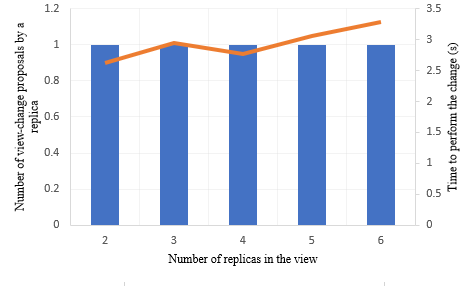
\includegraphics[width=1\linewidth]{images/pfd.png}
\caption{Number of view-change proposals and time until the view change is done in PFD.}
\label{fig:pfd}
\end{figure}

\begin{figure}[h]
\centering
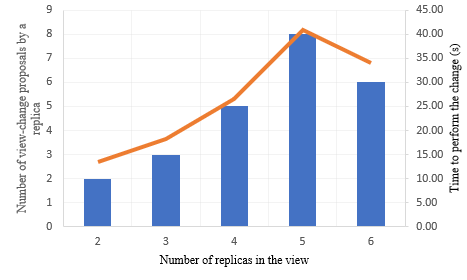
\includegraphics[width=1\linewidth]{images/ifd.png}
\caption{Number of view-change proposals and time until the view change is done in IFD.}
\label{fig:ifd}
\end{figure}

Figures \ref{fig:pfd} and \ref{fig:ifd} show the number of view-change proposals made
by a specific replica, when it starts to detect a faulty replica, until the view-change is completed successfully. As we can see, the PFD is pretty much constant, and it scales well with the number of replicas.
In the IFD, many proposals are made until all the replicas agree at relatively same time. This, however, can take a long
time or, on the contrary, be very quick. It depends on the circumstances of the asynchronous system. There is a tight correlation between the number of view-change proposals and the time it takes for a view change to be processed successfully:
the more proposals there are, the more time will pass until the view change is accepted by the quorum.

%------------------------------------------------------------------------- 
\SubSection{SMR vs XL}
In this section we'll discuss the main advantages of a variant in comparison with the other,
having in account the idiosyncrasies of each one.

The XL variant takes advantage of the semantics of the operations and improves the performance
as the \textit{add} and \textit{read} operations can be executed simultaneously. This doesn't 
happen in SMR, where each request is executed at its time in order to guarantee that all replicas execute them
in the same order. This sometimes results in the halt of the request execution because it didn't execute the previous one, 
which is not necessary in some cases (e.g. when there are two read requests). To verify the validity of this premise, we did a performance test with several clients performing read requests at the same time. We added a random delay between 10ms and 300ms.
\newline\newline
\fbox{\begin{minipage}{22em}
begin-repeat 200\\
add \textless{}"a",DADTestA(1,"b")\textgreater{}\\
read \textless{}"*",null\textgreater{}\\
end-repeat
\end{minipage}
}
\begin{figure}[h]
\caption{Client script for multiple reads and adds.}
\label{fig:manyreads_code}
\end{figure}

Each client performs 400 requests (add and read alternated), and the number of clients are incremented on each iteration (and so are the total
of requests). We used $f=1$.

\begin{figure}[h]
\centering
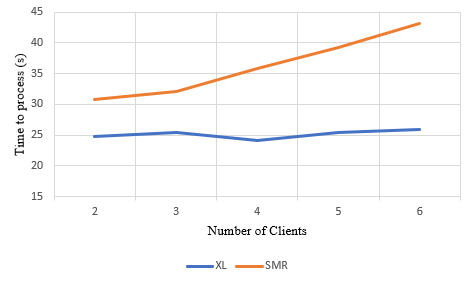
\includegraphics[width=1\linewidth]{images/manyreads.png}
\caption{Multiple reads in parallel.}
\label{fig:manyreads}
\end{figure}

In figure \ref{fig:manyreads}, although the number of requests is increasing, the XL variant keeps processing
the read requests almost at the same time. In contrast, in SMR, it takes longer to execute 
as the number of requests increases. 

SMR has an advantage in comparison with XL in the take operation. As explained in Xu-Liskov's paper~\cite{Xu1989ADF}, the take operation is like a two-phase commit. A client asks the replicas to lock all the tuples that match the given pattern and the replicas return them. If successful, the client does the intersection of all replicas' responses and, if not empty, selects the tuple to take and broadcasts to every other replica.
The bottleneck in this approach is the lock operation. The lock fails when it tries to lock an already locked tuple. So, if many clients attempt to take the same tuple pattern, the system will struggle so hard, that it would be better to have total order.
\newline\newline
\fbox{\begin{minipage}{22em}
begin-repeat 50\\
add \textless{}"a",DADTestA(1,"b")\textgreater{}\\
end-repeat\\
begin-repeat 50\\
take\textless{}"*",null\textgreater{}\\
end-repeat
\end{minipage}
}
\begin{figure}[h]
\caption{Client script for multiple take operation.}
\label{fig:manytakes_code}
\end{figure}

\begin{figure}[h]
\centering
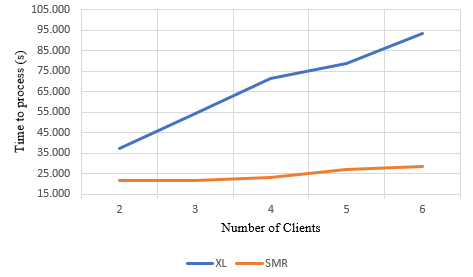
\includegraphics[width=1\linewidth]{images/manytakes.png}
\caption{Multiple takes in parallel.}
\label{fig:manytakes}
\end{figure}

In figure \ref{fig:manytakes} we can see how poorly XL performs when there are multiple 
take requests working with the same tuple set. In this case we used the same tuple, however that was just
a simple example of the problem. A tuple pattern can generate a huge set of tuples that match. So, even if
two clients are working with different tuple patterns, there might be a conflict if they sets intersect. In this case, both can fail to acquire a lock to their set.

In SMR, on the other hand, this isn't a problem. The requests are ordered and executed strictly in that agreed sequence, so, there aren't these type of conflicts.


%------------------------------------------------------------------------- 
\Section{Conclusion} \label{conclusion}
This paper presented two approaches for the implementation of a distributed fault-tolerant Tuple Space system. We
described the used algorithms and their implementation meticulously. In section \ref{evaluation} we verified that each variant's performance depends on the provided workload. 
For systems that require a higher availability, XL might, in general, be a better option, since it doesn't require total order, unlike SMR. 
However, if there is a high amount of removals (\textit{take} requests), SMR may outperform XL, especially if this type of operations are performed on tuple sets that intersect with each other.

Regarding failure detection, PFD will perform better if the network is stable. In the opposite case, where the network's health is impaired by the existence of partitions, big delays, or partial shutdowns, PFD might generate a lot of false positives, and non-faulty servers may wrongly leave the view, compromising the availability. In this case, IFD would be a safer choice.

%------------------------------------------------------------------------- 
\bibliographystyle{latex8}
\bibliography{latex8}

\end{document}

